% beamer class
\documentclass{beamer}

% load all packages
% input encoding
\usepackage[utf8]{inputenc}

% output font encoding
\usepackage[T1]{fontenc}

% package for the English language
\usepackage[english]{babel}

% default graphics path
\graphicspath{{logos/}{figures/}}

% package to create diagrams and plot with TikZ
\usepackage{pgfplots}
% always use the newest version
\pgfplotsset{compat=newest}
% define the style of the connection of two lines
\pgfplotsset{every axis/.append style={line join=bevel}}
% generate a new style template
\mode<beamer>{
	\pgfplotsset{
		beamer/.style={
			width=0.8\textwidth,
			height=0.45\textwidth,
			legend style={font=\scriptsize},
			tick label style={font=\footnotesize},
			label style={font=\small},
			max space between ticks=28,
		}
	}
}
\mode<handout>{
	\pgfplotsset{
		beamer/.style={
			width=0.8\textwidth,
			height=0.45\textwidth,
			legend style={font=\scriptsize},
			tick label style={font=\footnotesize},
			label style={font=\small},
			max space between ticks=25,
		}
	}
}
\mode<article>{
	\pgfplotsset{
		beamer/.style={
			width=0.8\textwidth,
			height=0.45\textwidth,
			max space between ticks=35,
		}
	}
}
% format and size template for two plots side-by-side
\pgfplotsset{
	scriptsize/.style={
		width=0.34\textwidth,
		height=0.1768\textwidth,
		legend style={font=\scriptsize},
		tick label style={font=\scriptsize},
		label style={font=\footnotesize},
		title style={font=\footnotesize},
		every axis title shift=0pt,
		max space between ticks=25,
		every mark/.append style={mark size=7},
		major tick length=0.1cm,
		minor tick length=0.066cm,
	}
}
\pgfplotsset{
	small/.style={
		width=6.5cm,
		height=,
		tick label style={font=\footnotesize},
		label style={font=\small},
		legend style={font=\footnotesize},
		max space between ticks=30,
	}
}
% align legends entries to the left
\pgfplotsset{legend cell align=left}
% draw a main grid
\pgfplotsset{xmajorgrids}
\pgfplotsset{ymajorgrids}
% number of minor ticks between two major tickmarks
%\pgfplotsset{minor x tick num={3}}
%\pgfplotsset{minor y tick num={3}}
% draw a minor grid
%\pgfplotsset{xminorgrids}
%\pgfplotsset{yminorgrids}
% scale only the axis using a certain width and height
\pgfplotsset{scale only axis}
% define colors like in MATLAB
\definecolor{matlab1}{rgb}{0,0,1}
\definecolor{matlab2}{rgb}{0,0.5,0}
\definecolor{matlab3}{rgb}{1,0,0}
\definecolor{matlab4}{rgb}{0,0.75,0.75}
\definecolor{matlab5}{rgb}{0.75,0,0.75}
\definecolor{matlab6}{rgb}{0.75,0.75,0}
\definecolor{matlab7}{rgb}{0.25,0.25,0.25}
% define a color cycle list like in MATLAB
\pgfplotscreateplotcyclelist{matlab}{
	{matlab1,solid},
	{matlab2,dashed},
	{matlab3,dashdotted},
	{matlab4,dotted},
	{matlab5,densely dashed},
	{matlab6,densely dashdotted},
	{matlab7,densely dotted}%this prevents an error
}
% use the earlier defined color list
\pgfplotsset{cycle list name=matlab}
% use the standard color list of pgfplots
%\pgfplotsset{cycle list name=color list}
% use only grayscale lines
%\pgfplotsset{cycle list name=linestyles}
% use a line width of 1pt
\pgfplotsset{every axis plot/.append style={line width=1pt}}
% use a comma as the dot separator for german documents
\addto\extrasngerman{\pgfplotsset{/pgf/number format/.cd,set decimal separator={{{,}}}}}
% use a half space as the 1000 separator
\pgfplotsset{/pgf/number format/.cd,1000 sep={\,}}
% define legend positions
\pgfplotsset{/pgfplots/legend pos/north/.style={/pgfplots/legend style={at={(0.50,0.97)},anchor=north}}}
\pgfplotsset{/pgfplots/legend pos/south/.style={/pgfplots/legend style={at={(0.50,0.03)},anchor=south}}}
\pgfplotsset{/pgfplots/legend pos/east/.style={/pgfplots/legend style={at={(0.97,0.50)},anchor=east}}}
\pgfplotsset{/pgfplots/legend pos/west/.style={/pgfplots/legend style={at={(0.03,0.50)},anchor=west}}}
\pgfplotsset{/pgfplots/legend pos/outer north/.style={/pgfplots/legend style={at={(0.50,1.03)},anchor=south}}}

% package for SI units
\usepackage[binary-units]{siunitx}
% real fractions
\sisetup{per-mode=fraction,mode=math}
% decimal marker in dependence from the language
\addto\extrasngerman{\sisetup{output-decimal-marker={,}}}
\addto\extrasenglish{\sisetup{output-decimal-marker={.}}}
% range phrase in dependence from the language
\addto\extrasngerman{\sisetup{range-phrase={ bis~}}} 
\addto\extrasenglish{\sisetup{range-phrase={ to~}}}

% A stand-alone package that implements several commands for including external animation and sound
% files in a pdf document. The package can be used together with both dvips plus ps2pdf and pdflatex,
% though the special sound support is available only in pdflatex.
\usepackage{multimedia}

% package to dissable floating in the article mode
\usepackage{float}

% package to change the line spacing
\usepackage{setspace}

% package for nice fractions in the text mode
\usepackage{xfrac}
% default with with a slash as in the usual math mode
\UseCollection{xfrac}{plainmath}

% nicer tables
\usepackage{booktabs}

% nicer quotation marks
\usepackage{csquotes}

% define labeling environment
\makeatletter
\newenvironment{labeling}[2][]{%
  \def\sc@septext{#1}%
  \list{}{\settowidth{\labelwidth}{{%
        #2%
          \sc@septext%
      }}%
    \leftmargin\labelwidth \advance\leftmargin by \labelsep
    \let\makelabel\labelinglabel
  }%
}{%
  \endlist
}
\newcommand\labelinglabel[1]{%
  #1\hfil
    \sc@septext%
}
\makeatother

% BibLaTeX package for direct citations
\usepackage[%
	style=ieee,%				format as used at the IEEE
	backend=biber,%			suppress warning
]{biblatex}

% database of references
\addbibresource{literature.bib}

\usepackage{url}
\usepackage{wrapfig}
% style of the Chair for Electromagnetic Compatibility
%\usepackage{beamer_emc}
% style of the Institute for Medical Engineering
%\usepackage{beamer_imt}
% style of the Faculty of Electrical Engineering and Information Technology
%\usepackage{beamer_feit}
% style of the Otto-von-Guericke-University
\usepackage{beamer_ovgu}
% style of STIMULATE (Solution Centre for Image Guided Local Therapies)
%\usepackage{beamer_stimulate}


\title[Short Title]{Academic Writing Using \LaTeX}
\author{Dias, Isabela P. L. \inst{1}}
\institute[]{
	\inst{1}%
	Institute of Physics, University of São Paulo (USP)\\
	Group Quantum Foundations
}
	\bibliography{references.bib}

\mode<presentation>{\keywords{Put some keywords here, separated by commas, e.g. Non-Technical Project, Academic Writing}}
\date[11/07/2022]{July 11th, 2022}

\begin{document}

\begin{frame}
	\maketitle
	% \maketitle also works in the article mode
	% \titlepage only works for presentation
\end{frame}
\subsection*{}

\begin{frame}
	\frametitle<presentation>{Introduction}
	\begin{block}{Welcome!}
	\begin{figure}
		\centering
			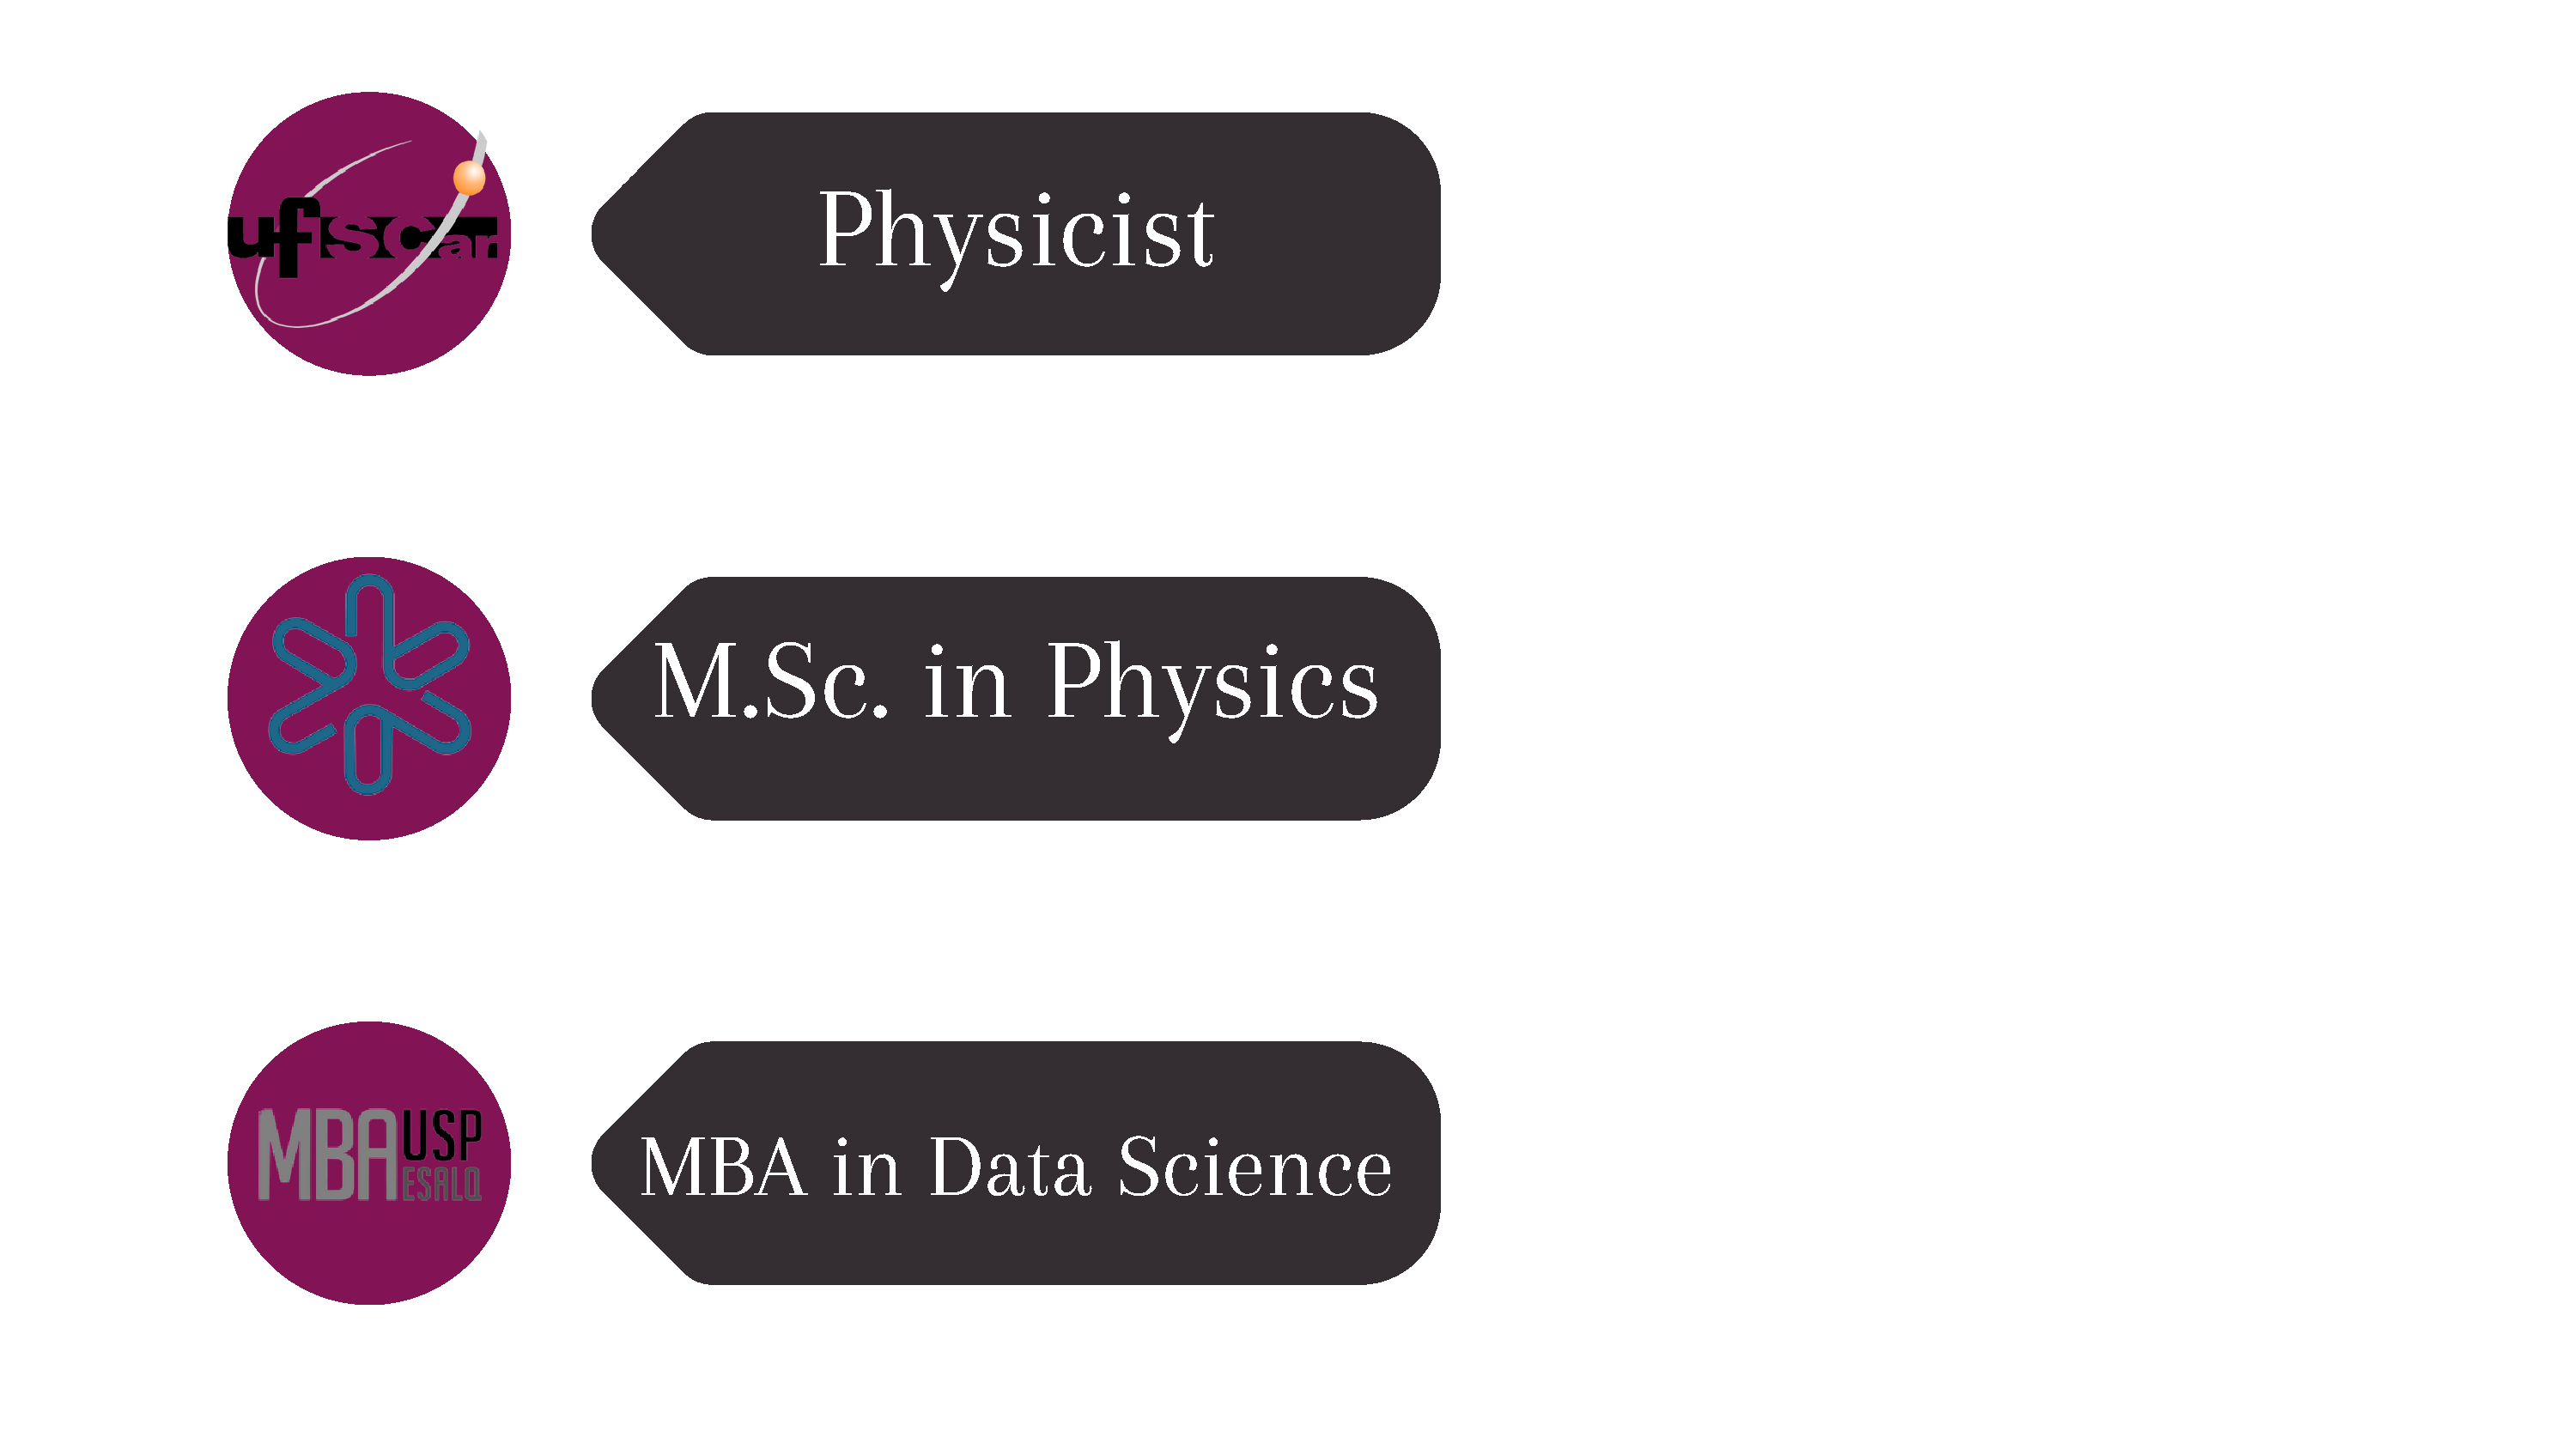
\includegraphics[height=5cm]{figures/timeline.pdf}
		\caption{My academic journey.}
		\label{fig:unilogo}
	\end{figure}
	\end{block}
\end{frame}
\subsection*{}

\begin{frame}
	\frametitle<presentation>{Introduction}
	\begin{block}{Objective:}
		\begin{itemize}
			\item \LaTeX \quad as a tool to write academic texts or lecture notes \nocite{Sasha}\nocite{Gray2003}
		\end{itemize}
	\end{block}
	\begin{block}{Pronounce \LaTeX ~}
		\begin{itemize}
			\item "LAY-TECH"
		\end{itemize}
	\end{block}
\end{frame}

\begin{frame}[label=inhalt]{Overview}
	\tableofcontents
\end{frame}

\section{Introduction}

% only for the miniframe navigation

\subsection*{}

\begin{frame}
	\frametitle<presentation>{Questions}
	\begin{block}{Time for questions:}
		\begin{figure}
		\centering
			
\includegraphics[height=5cm]{figures/questionstime.pdf}
		\label{fig:questions}
	\end{figure}
	\end{block}
\end{frame}

\section{What is \LaTeX?}

\subsection*{}

\begin{frame}
	\frametitle<presentation>{What is \LaTeX?}
	\begin{block}{\LaTeX is ...}
	\begin{itemize}
	    \item \textbf{Sophisticated} Software system for document preparation
	    \item Specific programming language to write INPUT file,
	    \item Program to interpret and compile the OUTPUT file,
	    \item Highest typographical quality and professional layout.
	\end{itemize}
		\begin{figure}
		\centering
			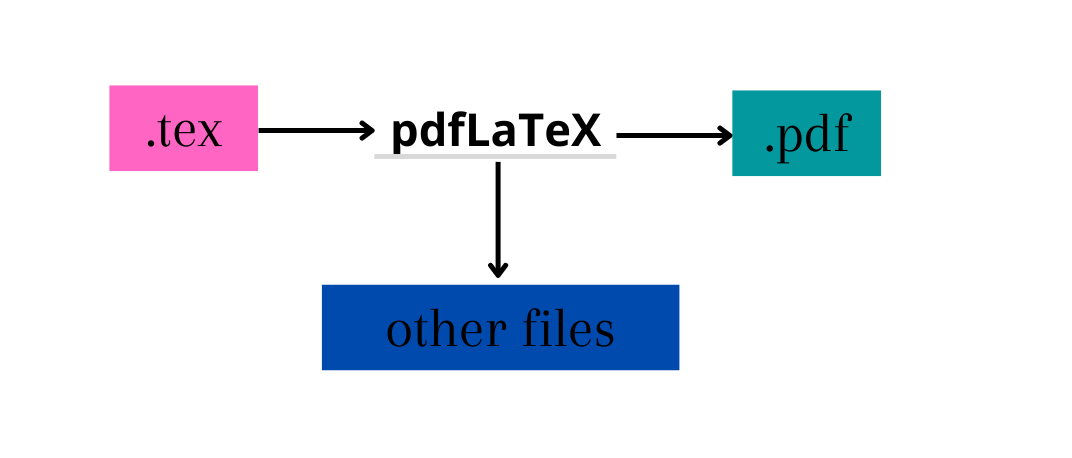
\includegraphics[height=3cm]{tex.png}
		\label{fig:texfile}
	\end{figure}
 	\end{block}
\end{frame}

\subsection{History}
%put that Leslie Lamport was the first developer and make a first manual
\begin{frame}
	\frametitle<presentation>{Brief history}
	\begin{figure}
		\centering
			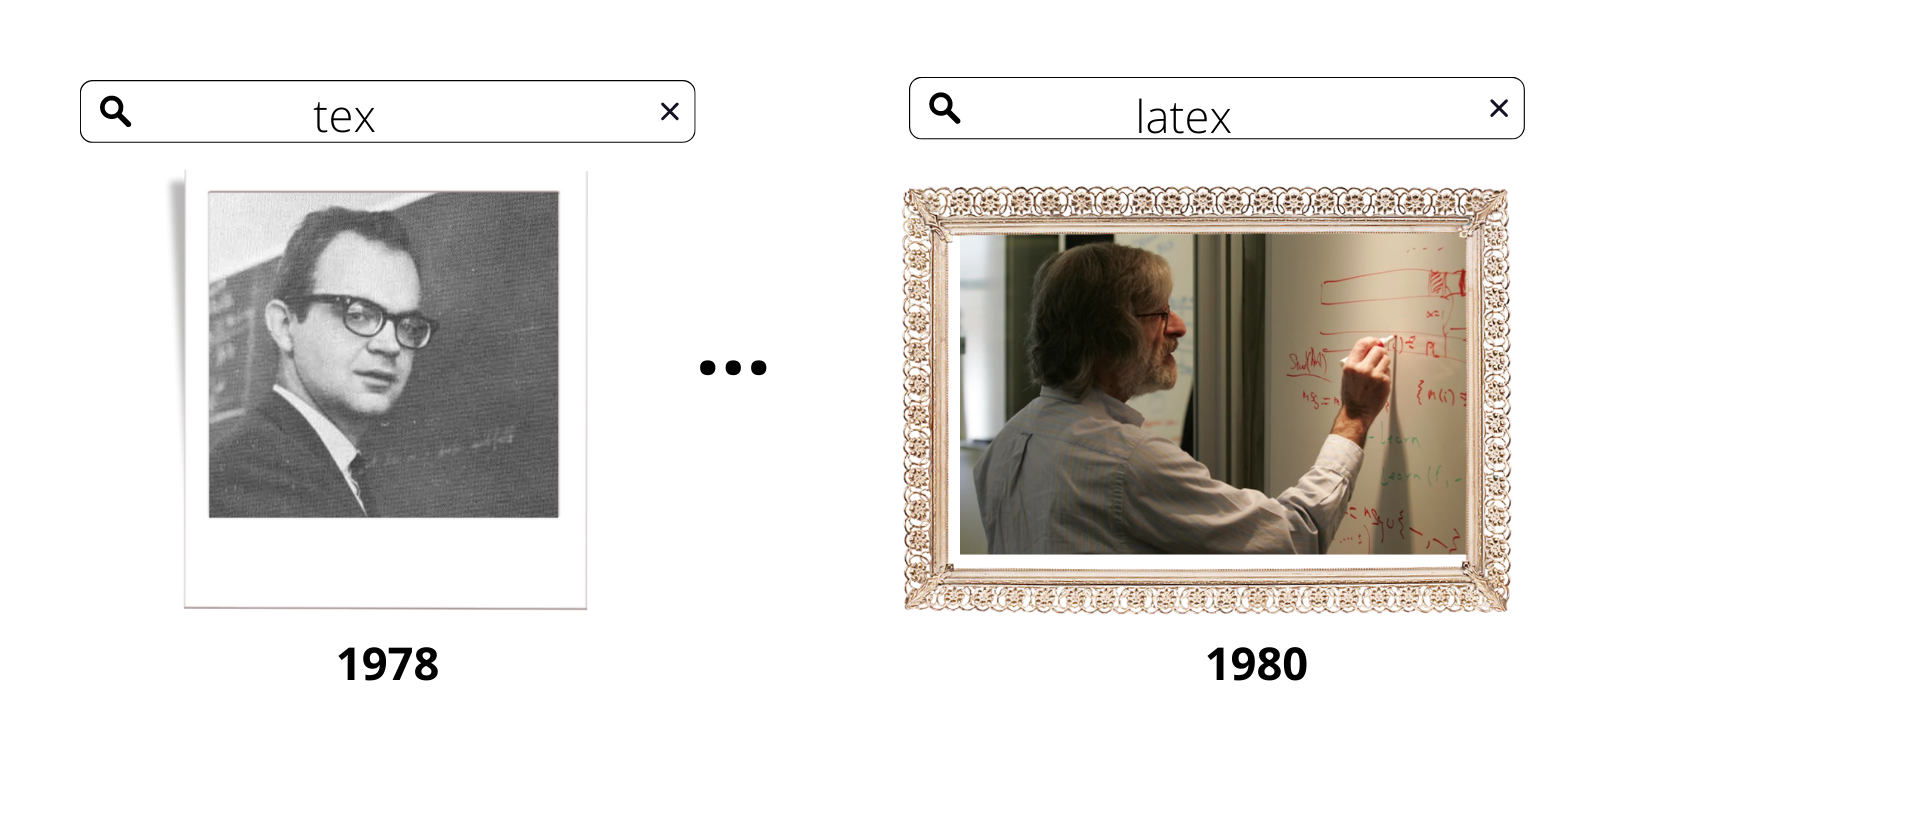
\includegraphics[height=5cm]{figures/texcreators.png}
		\caption{Donald Knuth and Leslie Lamport.}
		\label{fig:creators}
	\end{figure}
\end{frame}
\subsection*{}

\begin{frame}
	\frametitle<presentation>{How does it \textbf{look}?}
	\begin{block}{\textbf{Article} class}
		\begin{figure}
		\centering
			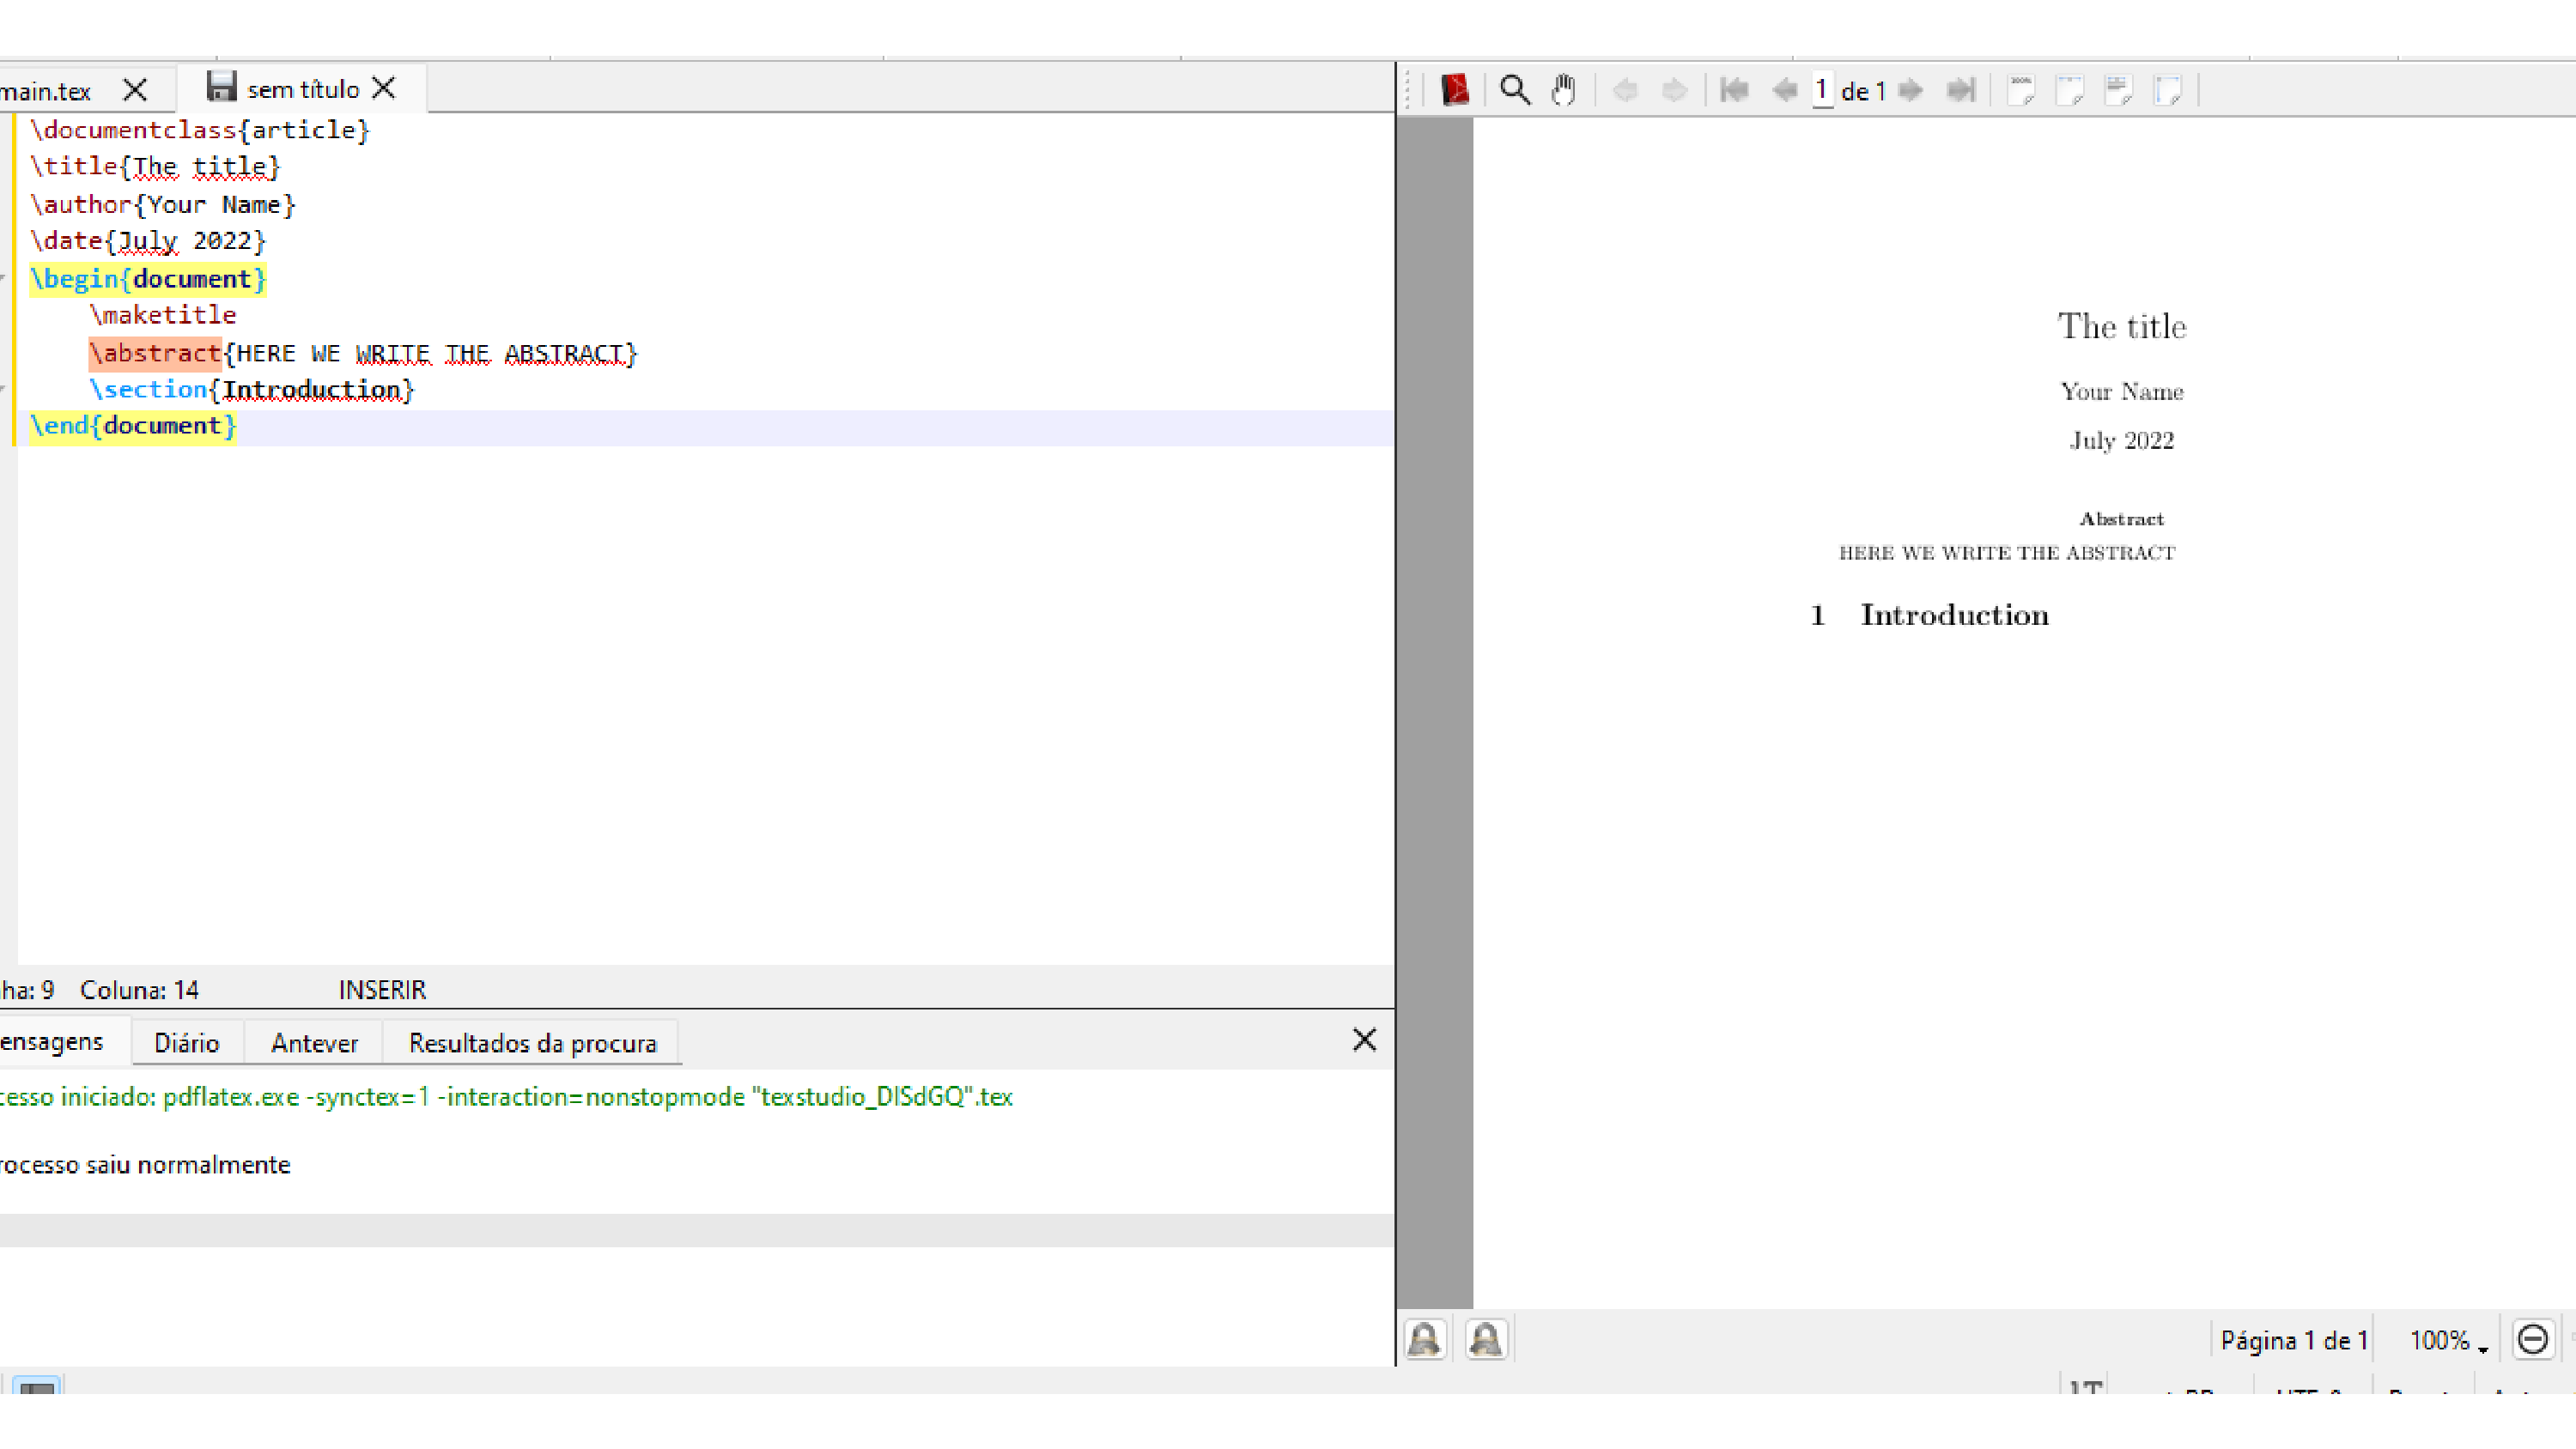
\includegraphics[height=6cm]{figures/lookslike.pdf}
		\label{fig:texfile}
	\end{figure}
 	\end{block}
\end{frame}



\subsection*{}

\begin{frame}
	\frametitle<presentation>{How does it \textbf{look}?}
	\begin{block}{\textbf{Formal Letter} class}
		\begin{figure}
		\centering
			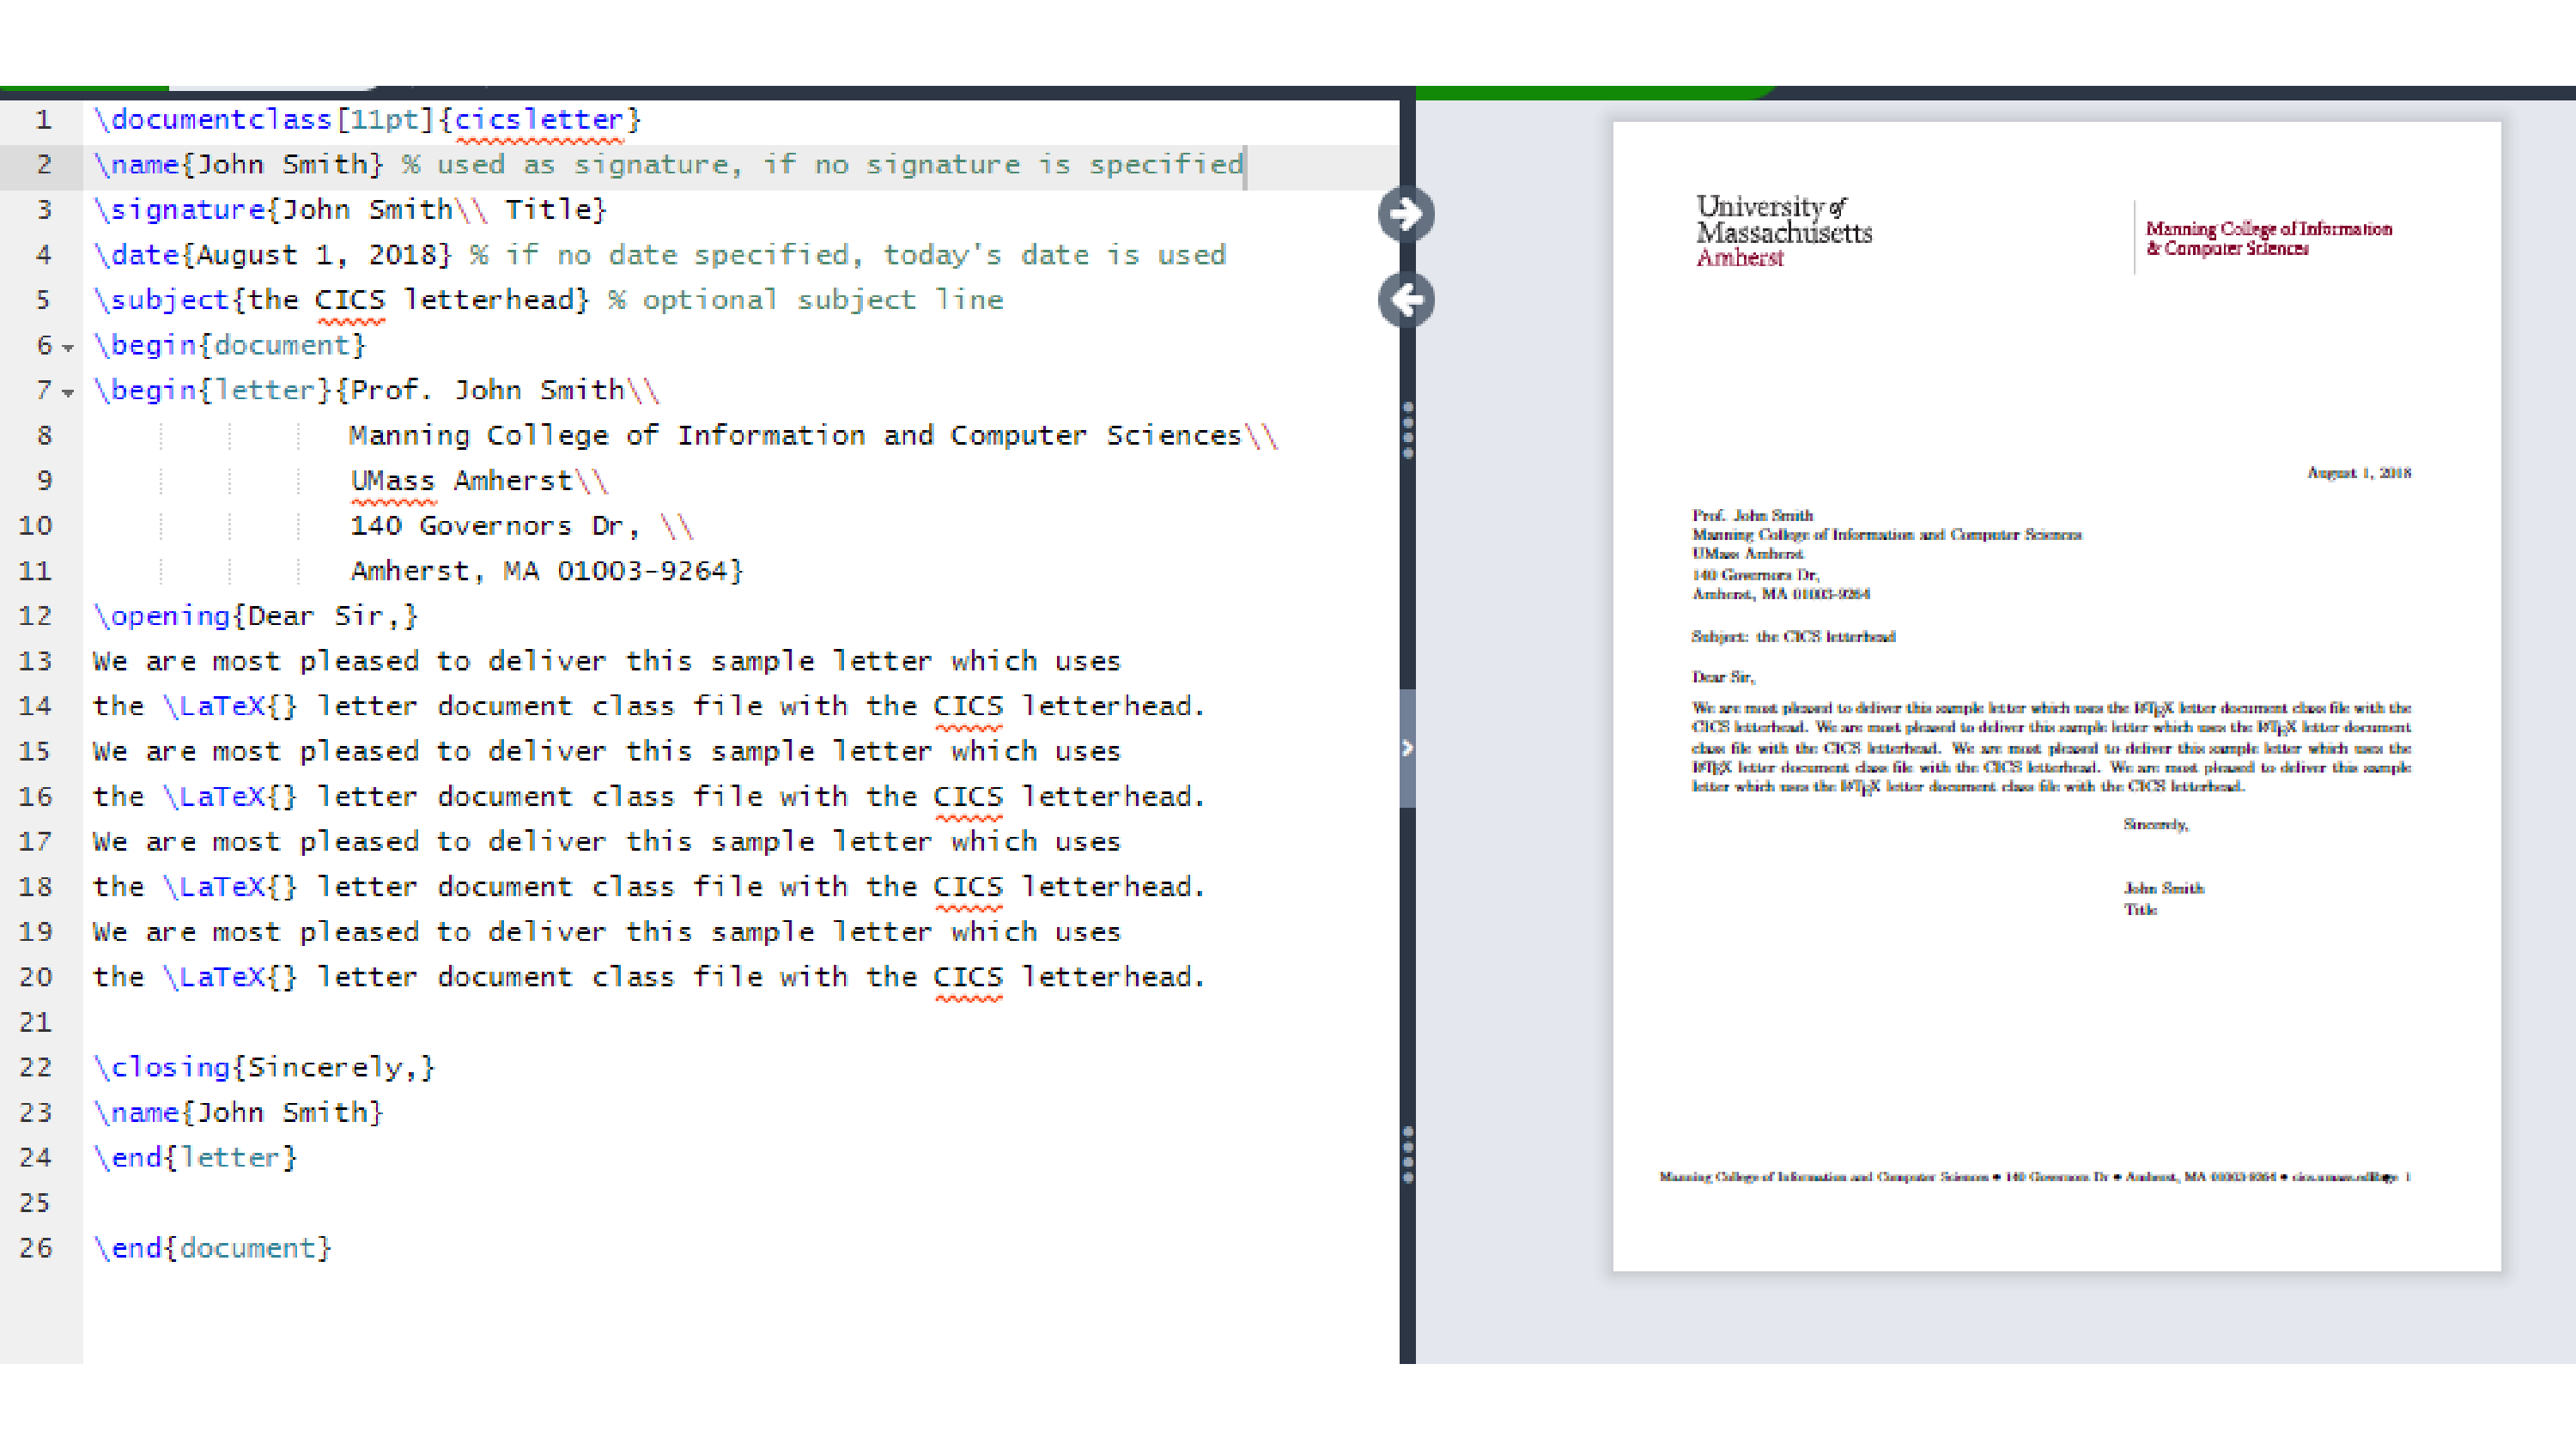
\includegraphics[height=6cm]{figures/lookslike2.pdf}
		\label{fig:texfile}
	\end{figure}
 	\end{block}
\end{frame}

\subsection*{}

\begin{frame}
	\frametitle<presentation>{Basic \textbf{commands}}
	\begin{block}{\textbf{Footnotes, Table of Contents, Bibliography}}
		\begin{figure}
		\centering
			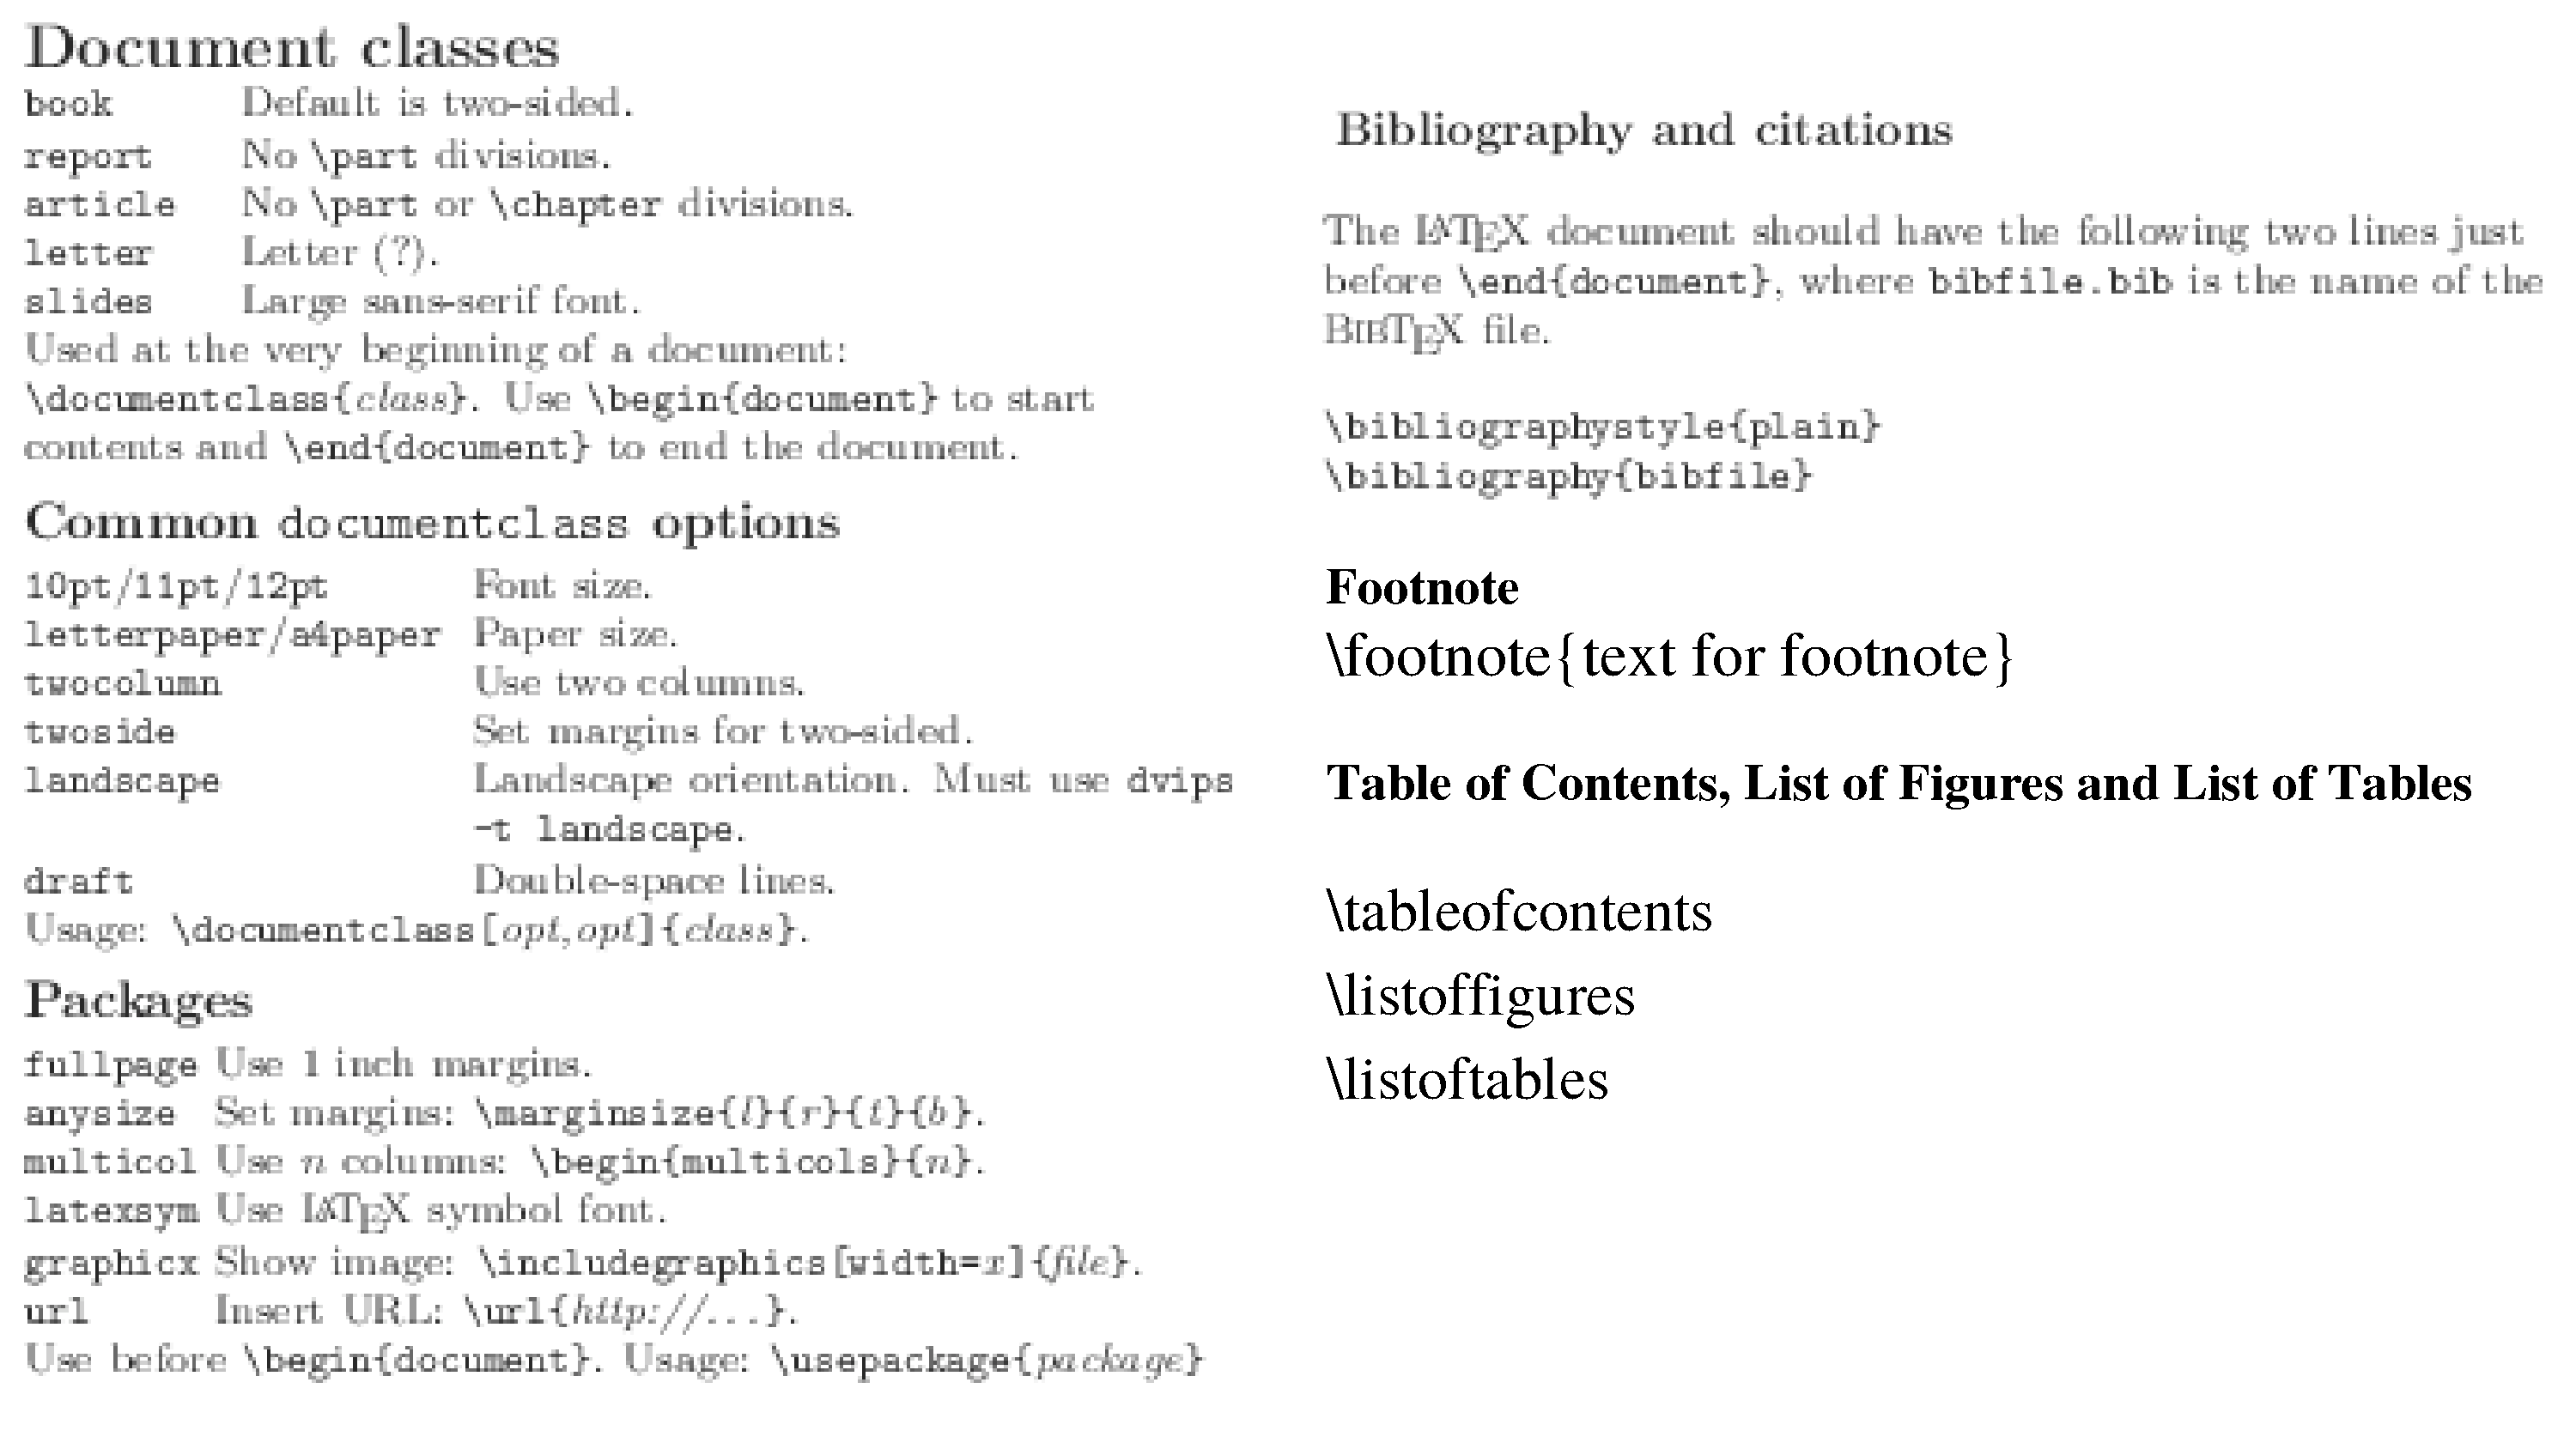
\includegraphics[height=6cm]{figures/basiccommands.pdf}
		\label{fig:texfile}
	\end{figure}
 	\end{block}
\end{frame}

\begin{frame}
	\frametitle<presentation>{Graphs and Equations}
		\begin{figure}
		\centering
			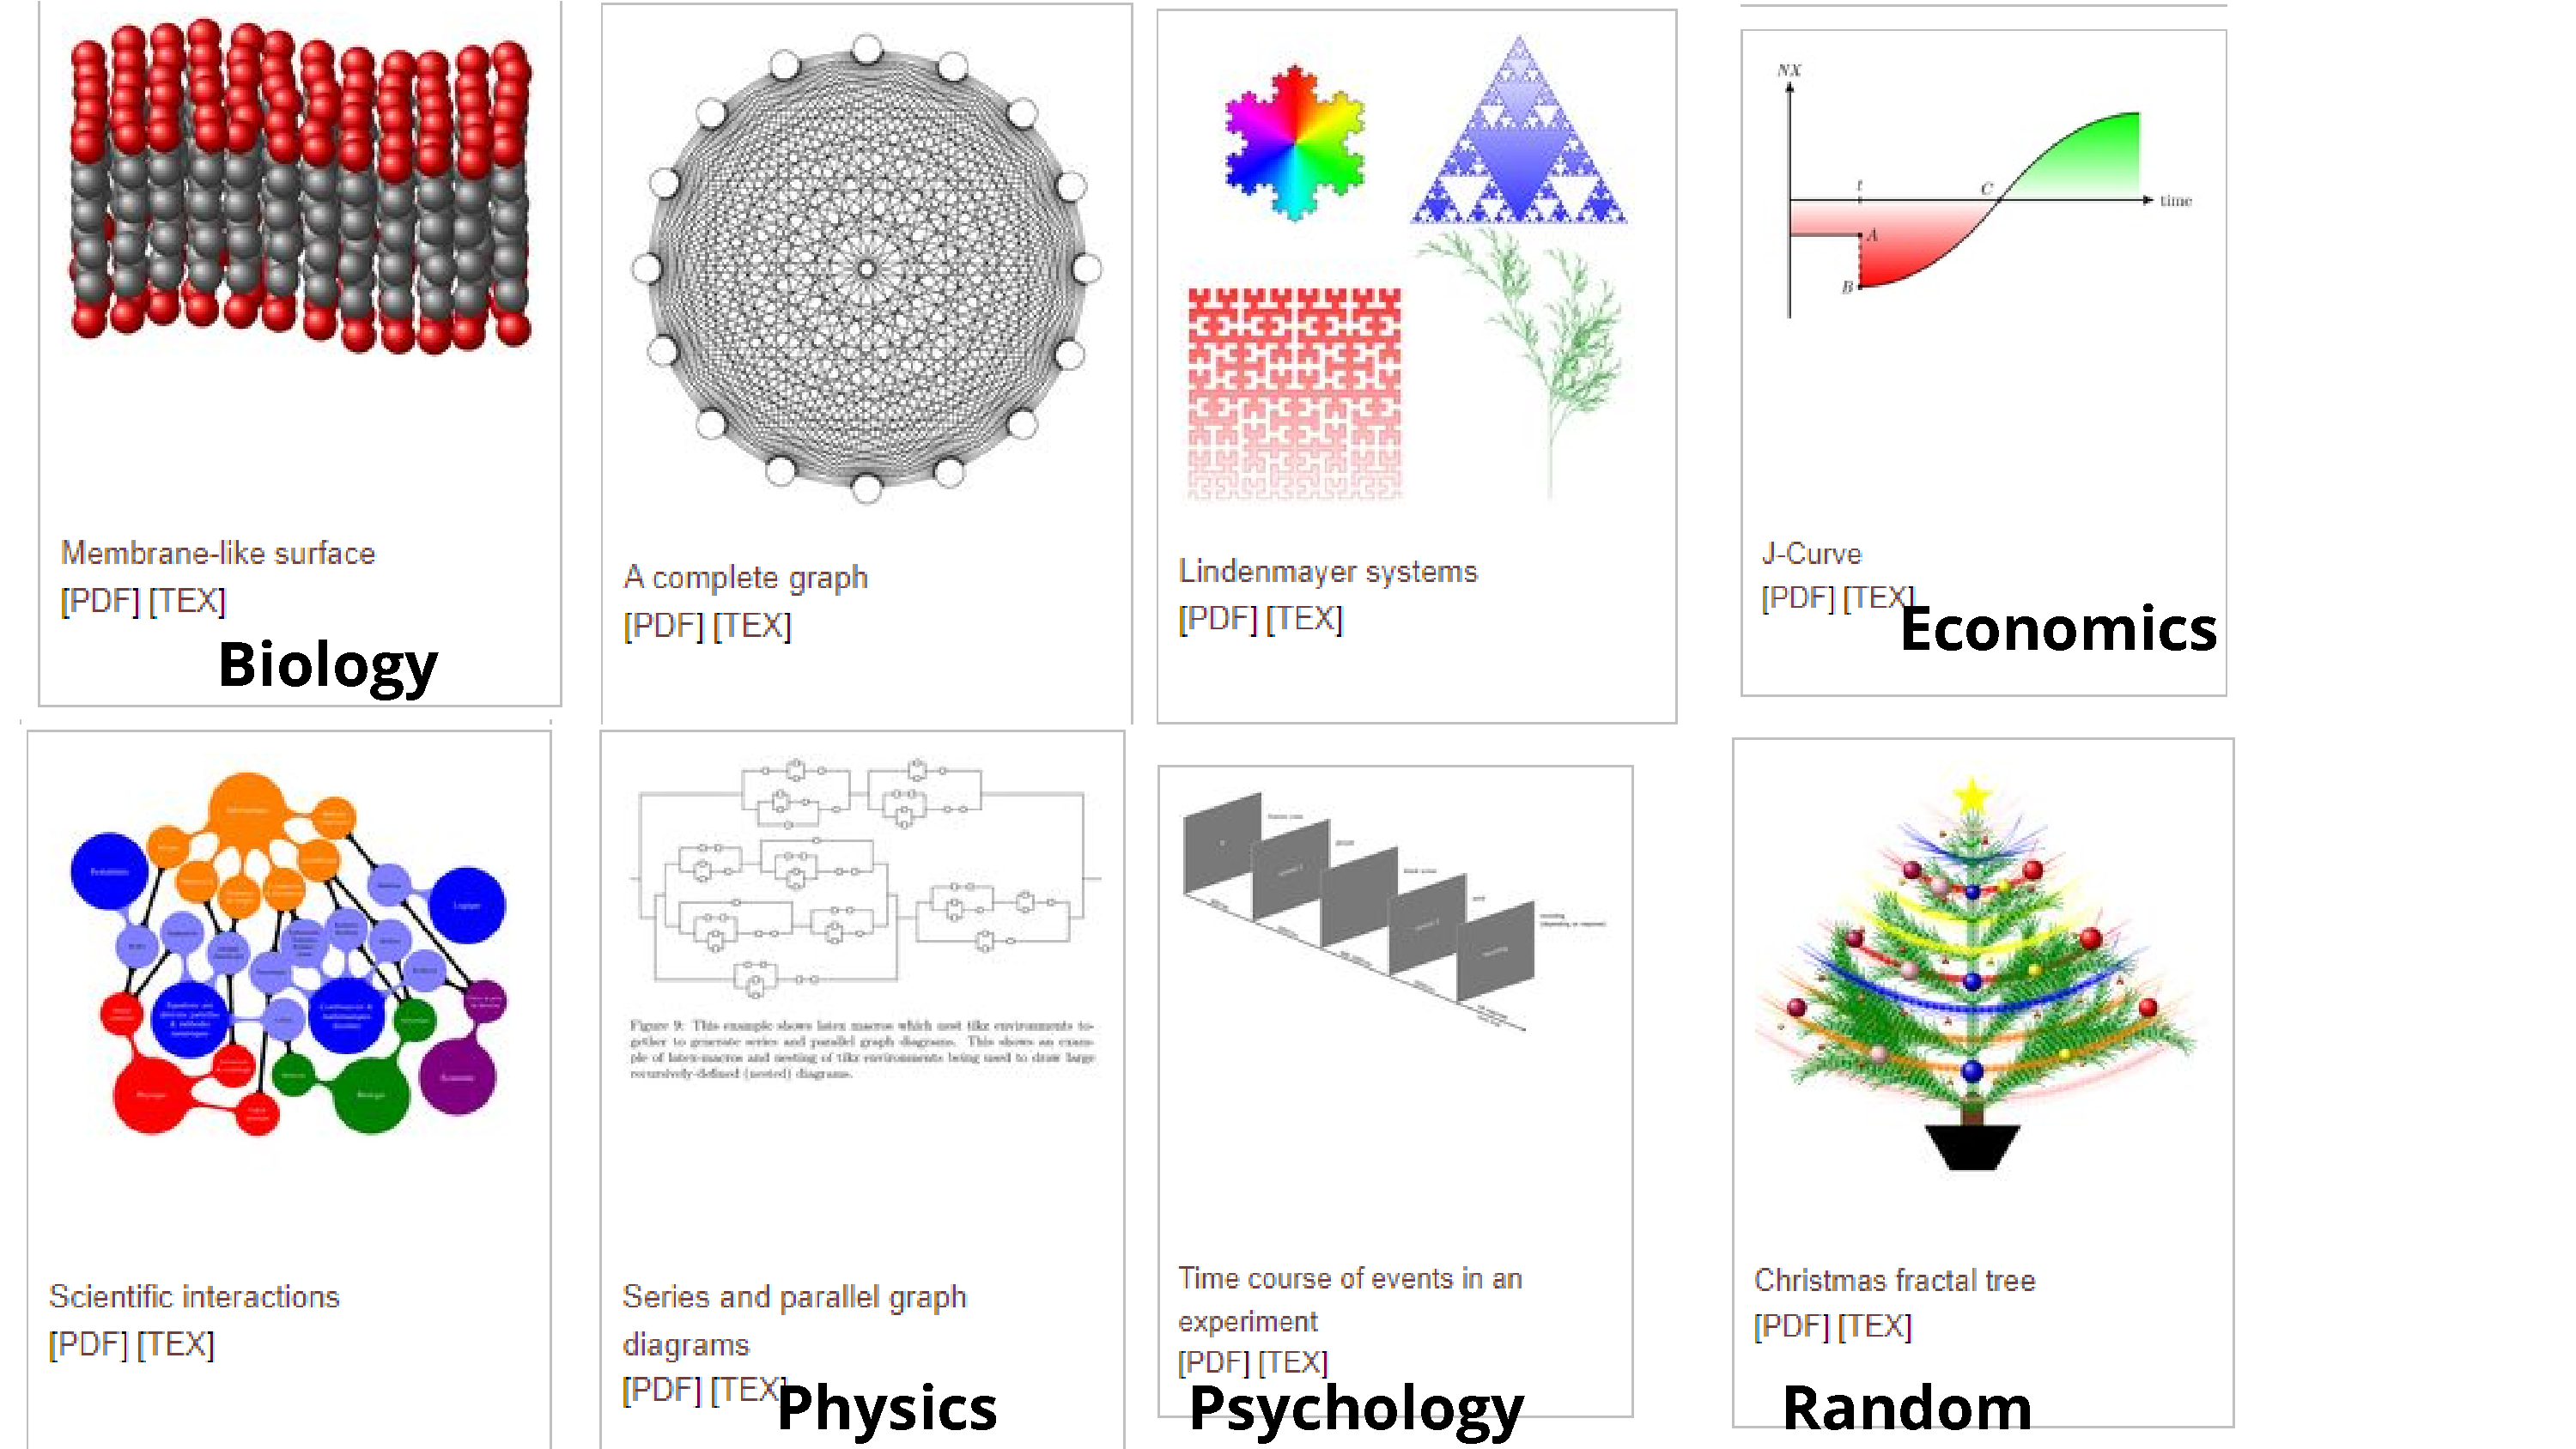
\includegraphics[height=6cm]{figures/graphs.pdf}
		\label{fig:graphs}
	\end{figure}
%	\begin{figure}
%		\centering
%			\begin{tikzpicture}
%				\begin{axis}[
%					beamer,
%					xlabel={time, $t$ (in \si{\milli\second})},
%					ylabel={voltage, $u(t)$ (in \si{\volt})},
%					xmin=0,xmax=20,
%					ymin=-350,ymax=350,
%					legend pos=south west,
%					% example how to insert a line by giving a formula directly
%					]
%					\addplot+[
%						domain=0:20,
%						samples=101,
%					] {sin(deg(x*2*pi/20))*sqrt(2)*230};
%					\addlegendentry{sine wave-form};
%					\addplot+[
%						domain=0:20,
%						samples=101,
%					] {cos(deg(x*2*pi/20))*sqrt(2)*230};
%					\addlegendentry{cosine wave-form};
%				\end{axis}
%			\end{tikzpicture}
%		\caption{Harmonic time course of a voltage with a frequency of \SI{50}{\hertz} 
%		and an effective value of \SI{230}{\volt}.}
%		\label{fig:u_t_sinus}
%	\end{figure}
\end{frame}

\subsection{Installation}

\begin{frame}{Installation}

	\begin{block}{Two steps are required}
	\begin{itemize}
	    \item \LaTeX distribution (MikTeX)
	    \item Plain Text Editor.
	    \item PDF Reader,
	    \item or \textbf{NOTHING}.
	\end{itemize}
	
 	\end{block}
\end{frame}

\subsection*{}

\begin{frame}{Installation}



\begin{wrapfigure}{r}{0.25\textwidth}

\includegraphics[width=0.9\linewidth]{figures/magically.png} 
\label{fig:wrapfig}
\end{wrapfigure}
	\begin{block}{\LaTeX distribution (MikTeX)}
	\end{block}
- Get a copy of MikTeX distribution from \url{https://miktex.org/}
	     
	   -  Install magically all packages. 
	     
	    - There are currently 5729 packages in the MiKTeX package repository.


\end{frame}
\subsection*{}
\begin{frame}{Installation}


\begin{wrapfigure}{r}{0.25\textwidth}

\includegraphics[width=0.9\linewidth]{figures/texstudio.png} 
\label{fig:wrapfig}
\end{wrapfigure}

\begin{block}{Plain Text Editor}
\end{block}
- Integrated writing environment for creating \LaTeX documents

- Syntax-highlighting,

- Integrated viewer,

- Reference checking.
    
\end{frame}
\subsection*{}
\begin{frame}{Installation}


\begin{wrapfigure}{r}{0.25\textwidth}

\includegraphics[width=0.9\linewidth]{figures/overleaf.png} 
\label{fig:wrapfig}
\end{wrapfigure}

\begin{block}{\textbf{Overleaf} -Remotely }
\end{block}

-  Collaborative cloud-based \LaTeX editor,

- Editor used for writing, editing and publishing scientific documents,

-  Provide official journal \LaTeX templates and direct submission links. 
    
\end{frame}



\subsection{Advantages}

\begin{frame}
	\frametitle<presentation>{Advantages}
\begin{block}{\textbf{Minimal} effort}
\begin{itemize}
    \item You only need to learn basic commands 
    \item Complex structures : Footnotes, references, table of contents and bibliography
    \item \LaTeX encourages authors to write well-sctructured texts
    \item Runs on almost any hardware platform avaiable.
\end{itemize}
\end{block}
\end{frame}
\subsection*{}

\begin{frame}
	\frametitle<presentation>{Disadivantages}
\begin{block}{\textbf{Logical} Structure}
\begin{itemize}
\item Frustration for beginners (at first glance)
 \item Markup language, the content is written in plain text and you can use commands to “order” how things should be displayed.
  
  
\end{itemize}
\end{block}
\end{frame}


%\begin{frame}{Citations}
	%\begin{block}{Don't use short citations:}
	%	\begin{itemize}
			%\item avoid short citations like~[1]
			%\item no one will remember the numbers when the list of %references is shown
%			\item use full citations instead
%		\end{itemize}
%	\end{block}
%	\begin{block}{Example for a full citation:}
%		\small\fullcite{hering:technical_reports}
%	\end{block}
%\end{frame}

\section{Conclusion}

% only for the miniframe navigation
\subsection*{}

\begin{frame}
	\frametitle<presentation>{Conclusion}
	\begin{block}{Results:}
	  \begin{itemize}
	  	\item Very useful for academic work, especially at the graduate level,
	  	\item Most advanced math typesetting systems
	  	\item \LaTeX allows you to make more consistent and more easily changeable documents
		\end{itemize}
	\end{block}
\end{frame}

% only for the miniframe navigation
\subsection*{}
\begin{frame}
	\frametitle{Bibliography}
	\printbibliography
\end{frame}

\section*{}

\begin{frame}<beamer>{}
	\begin{center}
		Thanks for your attention!
	\end{center}
	\begin{center}
		Are there questions?
	\end{center}
\end{frame}

\end{document}
